\chapter{Vektorraumbündel}\lecture 

\incfig{3}{14cm}

\begin{defn}[Vektorraumbündel]\index{Vektorraumbündel}
	Ein (reelles topologisches) \emph{Vektor(raum)bündel} von Rang $n$ über $B$ ist ein Tripel $(E,\pi,B)$, wobei $E$ ("Totalraum") und $B$ ("Basis") topologische Räume sind und $\pi: E \to B$ stetig, surjektiv und so ist, dass gilt:
	\begin{enumerate}[label={\roman*})]
		\item $\foralll x \in B$ ist das Urbild $\pi^{-1}(x) =: E_x$ ("Faser über $x$") ein $n$-dimensionaler Vektorraum (über $\R$)
		\item $\foralll x \in B \ \exists$ offene Umgebung $U$ von $x$ und ein Homöomorphismus $\psi: \overbrace{\pi^{-1} (U)}^{\in \bound{E}{U}} \to U \times \R^n$, sodass $\pi = pr_1 \circ \psi$ ($pr_1 =$ Projektion auf den ersten Faktor, also $U$) und sodass $\psi_y = \bound{\psi}{E_y} : E_y \to \{y\} \times \R^n \ \foralll y \in U$ ein Vektorraum-Isomorphismus ist ("lokale Trivialität"). $(\psi,U)$ heißt "lokale Trivialisierung" oder "\emph{Bündelkarte}".
	\end{enumerate}
\end{defn}

\begin{minipage}{\linewidth}
	\begin{wrapfigure}{R}{8cm}
		\centering
%		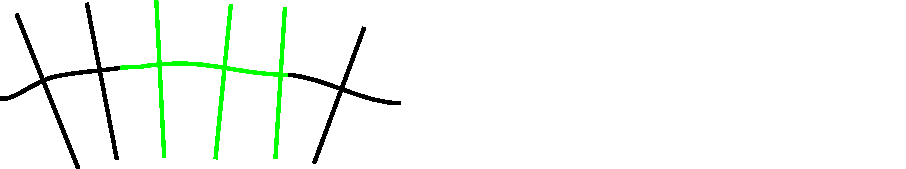
\includegraphics[width=8cm]{3_1 kart}
		\wrapincfig{3_1 kart}{8cm}
	\end{wrapfigure}

	Das heißt lokal lässt sich ein Bündel auffassen als karthesisches Produkt. Gibt es eine globale Trivialisierung (also $(\psi,U)$ Bündelkarte mit $U = B$), so heißt das Bündel \emph{trivial}.
\end{minipage}

\begin{exmp*}
	\begin{enumerate}[label = {\roman*})]
		\item 	Zylinder: $ \Sbb^1 \times \R \to \Sbb^1 $ ist trivial
			\incfig{3_1 zylinder}{2cm}
		\item "Unendlich ausgedehntes" Möbiusband  $ \pi: E \to \Sbb^1 $ von Rang 1, ein nicht triviales Bündel über $\Sbb^1$ mit Faser $\cong \R$ (später mehr)
			\incfig{3_1 moebius}{8cm}
		\item $ N = \{(p,v) \in \Sbb^2 \times \R^3 \mid v \| p\}\ (\Sbb^2 \subset \R^3) $
			\incfig{3_1 buendel}{12cm}
			Das Normalenbündel ist trivial.
		\item \begin{minipage}{\linewidth}
				\begin{wrapfigure}{R}{5cm}
					\centering
					\wrapincfig{3_1 moebius2}{5cm}
				\end{wrapfigure}
				(vgl. Diff 2)
			\end{minipage} \\
			$ M = $ Möbiusband\\
			$ \pi^{-1}(x) = \{\lambda n_x \mid \lambda \in \R\} $\\
			$ x \mapsto n_x$ Einheitsnormalen-Vektorfeld\\
			Das Bündel ist nicht trivial. (später mehr)
	\end{enumerate}
\end{exmp*}

\begin{defn}[Schnitt]\index{Vektorraumbündel!Schnitt}
	Ein \emph{Schnitt} eines Vektorraumbündels $ (E,\pi,B) $ ist eine stetige Abbildung $ z: B \to E $ mit $z(x) \in E_x\ \foralll x \in B$.
	\incfig{3_2}{8cm}
\end{defn}
	
\begin{exmp*}
	Nullschnitt: $ B \to E,\ x \mapsto 0 \in E_x $
	\incfig{3_2 nullschnitt}{12cm}
\end{exmp*}

\begin{rem*}
	$ z: B \to E $ Schnitt $ \implies z: B \to z(B) $ Homöomorphismus.\\
	$z_0$ Nullschnitt: $z_0(B) \cong B$.
\end{rem*}

\begin{defn}[Bündelatlas, Übergangsfunktion]\index{Vektorraumbündel!Bündelatlas} \index{Vektorraumbündel!Übergangsfunktion}
	Sei $ (E,\pi,B) $ ein Vektorraumbündel von Rang $n$. Eine Menge von Bündelkarten $ \{(\varphi_\alpha, U_\alpha) \mid \alpha \in A\} $ heißt \emph{Bündelatlas} von $E$, wenn $ \bigcup_{\alpha \in A} U_\alpha = B. $
	Die auf Überlappungen $ U_\alpha \cap U_\beta $ gegebenen stetigen Abbildungen 
	$$ \Phi_{\alpha \beta}: U_\alpha \cap U_\beta \to \GL(n,\R),\ x \mapsto \bound{\varphi_\beta}{E_x} \circ \big( \bound{ \varphi_\alpha}{E_x} \big)^{-1} $$
	heißen \emph{Übergangsfunktionen}.
\end{defn}

\begin{rem*}
	$\Phi_{\alpha \beta}$ nehmen tatsächlich Werte in $\GL(n,\R)$ an:
	\incfig{3_3}{12cm}
	$$ \bound{\varphi_\beta}{E_x} \circ \big( \bound{\varphi_\alpha}{E_x} \big)^{-1}: \underset{\cong \R^n}{\{x \times \R^n\}} \to \underset{\cong \R^n}{\{x \times \R^n\}} $$
	ist ein Vektorraumisomorphismus für jedes $x$. (nach Definition Bündelkarte)
\end{rem*}

\begin{rem*}
	Es gilt die sogenannte \emph{Kozykelbedingung}:
	\incfig{3_3 kozykel}{14cm}
\end{rem*}

\begin{exmp*}
	$ \Sbb^1 \subset \R^2 $\\
	\begin{minipage}{\linewidth}
		\begin{wrapfigure}{R}{4cm}
			\centering
%			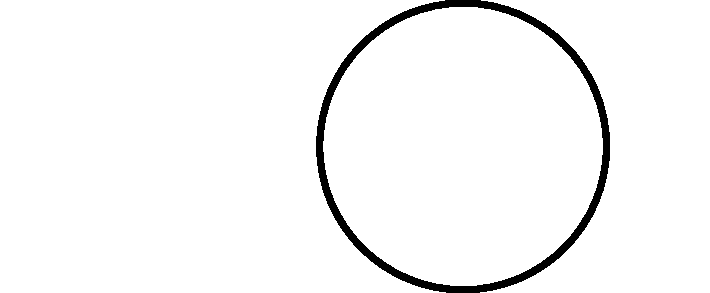
\includegraphics[width=4cm]{3_3 circ}
			\wrapincfig{3_3 circ}{4cm}
		\end{wrapfigure}
		$ U_1 = \Sbb^1 \setminus \{p_1\},\ U_2 = \Sbb^1 \setminus \{p_2\} $ (offen in $\Sbb^1$)\\
		überdeckt $\Sbb^1$: $ U_1 \cap U_2 = \bigg\{ \underset{V_+}{\bigcap}, \overset{V_-}{\bigcup} \bigg\} $\\
		Sind die Übergangsfunktionen $ \Phi_{21}(p) = \id_\R\ \foralll p \in U_1 \cap U_2 $, so ist das Bündel trivial. Denn dann kann man eine lokale Trivialisierung auf $ U \subset \Sbb^1 $ auf ganz $\Sbb^1$ fortsetzen. Man erhält den Zylinder.\\
		Wählen wir als Übergangsfunktion
		\begin{alignat*}{2}
			\Phi_{21}(p) &= \id_\R \qquad &&\foralll p \in V_+\\
			\Phi_{12}(p) &= -\id_\R \qquad &&\foralll p \in V_-
		\end{alignat*}
		erhält man das "Möbiusband" (unendlich ausgedehnt)
	\end{minipage}
	\incfig{3_3 geom}{15cm}
\end{exmp*}

\begin{defn*}
	Wie bei Mannigfaltigkeiten gilt: Ein Bündelatlas über einer differenzierbaren Mannigfaltigkeit heißt \emph{differenzierbar}, falls alle Übergangsfunktionen (als Funktionen von $p \in M = B$) glatt sind. Ein differenzierbares Vektorbündel ist ein Vektorbündel über $M$ mit einem maximalen differenzierbaren Bündelatlas.\\
	Eine Funktion $ f: E \to \tilde{E}\ (E,\tilde{E}$ differenzierbare Bündel) heißt differenzierbar/glatt in $p \in \pi(E)$, wenn $ \tilde{\varphi} \circ f \circ \varphi^{-1} $ differenzierbar/glatt in $\varphi(p)$ ist, wobei $(\varphi,U)$ eine Bündelkarte bei $p$ ist und $(\tilde{\varphi},\tilde{U})$ eine Bündelkarte bei $f(p)$ ist (jeweils aus dem maximalen differenzierbaren Bündelatlas). 
\end{defn*}

\begin{defn}[Prä-Vektorraumbündel, Prä-Bündelatlas] \index{Vektorraumbündel!Prä-Vektorraumbündel} \index{Vektorraumbündel!Prä-Bündelatlas}
	Ein \emph{Prä-Vektorraumbündel} ist ein Quadrupel $ (E,\pi,B,\Acal) $, wobei $E$ eine Menge ist, $B$ ein topologischer Raum, $\pi: E \to B$ surjektiv, sodass $E_x = \pi^{-1}(x)$ ein Vektorraum ist, und mit einem \emph{Prä-Bündelatlas} $\Acal$, das heißt einer Menge $ \{(\varphi_\alpha,U_\alpha) \mid \alpha \in A\} $, sodass $U_\alpha \subset B$ offen, $ B = \bigcup_{\alpha \in A} U_\alpha $ und $ \varphi_\alpha: \pi^{-1}(U) \to U \times \R^n $ bijektiv für alle $\alpha$, sodass $ \bound{\varphi_\alpha}{E_y}: E_y \to \{y\} \times \R^n $ ein Vektorraum-Isomorphismus ist und so, dass die Übergangsfunktionen 
	$ \begin{aligned}[t]
		\Phi_{\alpha \beta}: &U_\alpha \cap U_\beta \to \GL(n,\R),\\
		 &x \mapsto \bound{\varphi_\beta}{E_x} \circ \big( \bound{\varphi_\alpha}{E_x} \big)^{-1}
	\end{aligned} $ stetig sind.
\end{defn}

\begin{rem}
	\begin{enumerate}[label= {\roman*})]
		\item Sei ein Prä-Vektorraumbündel $ (E,\pi,B,\Acal) $ gegeben. Wie in Lemma \ref{1.14} zeigt man, dass eine Topologie auf $E$ (eindeutig!) dadurch festgelegt ist, dass man fordert, dass $(E,\pi,B)$ ein Vektorraumbündel ist und $\Acal$ ein Bündelatlas. (Man erklärt die Topologie so, dass die $\varphi_\alpha$ Homöomorphismen sind.)
		\item Ist $M$ eine differenzierbare Mannigfaltigkeit und $ (E,\pi,M,\Acal) $ ein differenzierbares Prä-Vektorraumbündel (das heißt alle Übergangsfunktionen sind glatt) erhält man auf diese Art sogar ein differenzierbares Vektorraumbündel (die differenzierbare Struktur ist eindeutig durch $\Acal$ festgelegt durch Übergang zu $\Dcal(\Acal)$).
	\end{enumerate}
\end{rem}

\begin{exmp}
	Sei $M$ eine differenzierbare $n$-dimensionale Mannigfaltigkeit. Sei $\Acal$ ein differenzierbarer Atlas von $M$. Dann ist $(TM, \pi, M, \Acal)$ mit
	\begin{align*}
		TM &= \bigcup_{p \in M} T_pM\\
		\pi&: TM \to M,\quad T_pM \mapsto p\\
		\Acal&= \Bigg\{ \begin{aligned}
			\varphi: \pi^{-1}(U) &\to U\times \R^n,\\
			 T_pM \ni X_p &\mapsto \big( p, X_p(\overbar{\varphi_1}), \dotsc, X_p(\overbar{\varphi_n}) \big)
		\end{aligned} \ \bigg|\ (\varphi,U) \in \Acal \Bigg\},
	\end{align*}
	wobei $ X_p (\overbar{\varphi_j}) = j $-te Koordinate von $X_p \in T_pM$ bezüglich $(\varphi,U)$ (vgl. Lemma \ref{2.7}),\\
	ein Prä-Vektorraumbündel.\\
	Das zugehörige differenzierbare Vektorraumbündel $TM$ über $M$ heißt das \emph{Tangentialbündel}. 
\end{exmp}

\begin{exmp*}
	$ T\Sbb^1 = \big\{(x,v) \in \Sbb^1 \times \R^2 \subset \R^4 \mid x \bot v \big\} $\\
	\begin{minipage}{\linewidth}
		\begin{wrapfigure}{R}{4cm}
			\centering
%			\includegraphics[width=4cm]{3_6}
			\wrapincfig{3_6}{4cm}
		\end{wrapfigure}
		$ \pi: T\Sbb^1 \to \Sbb^1,\ \pi(x,v) = x $\\
		globale Trivialisierung: $ T\Sbb^1 \to \Sbb^1 \times \R,\ (x,v) \mapsto (x,\lambda) $, wobei $\lambda v = \begin{pmatrix}
			-x_2\\x_1
		\end{pmatrix}$\\
		Das Bündel ist also trivial.
	\end{minipage}
\end{exmp*}

\begin{rem*}
	$ \varphi_2^+ : U_2^+ \cap \Sbb^1 \to \R,\ \varphi_2^+(x_1,x_2) = x_1 $
	\begin{align*}
		X_{\gamma,x}\big( \overbar{\varphi_2^+} \big) &= \frac{d}{dt} \big( \overbar{\varphi_2^+} \circ \overbar{\gamma} \big) (0)\ \text{mit} \begin{aligned}[t]
			&\gamma: (-\epsilon,\epsilon) \to \Sbb^1\\
			&\gamma(0) = x\\
			&\gamma(t) = (\cos(t+\alpha),\sin(t+\alpha))
		\end{aligned}\\
		&= \begin{pmatrix}
			-\sin(\alpha) \\ \cos(\alpha)
		\end{pmatrix}
	\end{align*}
	Bündelkarte: $\varphi_{2,+}: \pi^{-1}(U_2^+ \cap \Sbb^1) \to U_2^+ \cap \Sbb^1 \times \R,\ \varphi_{2,+}(\underbrace{X_{p,x}}_{\in Tx\Sbb^1}) = \big( x, X_{\gamma,x}\big( \overbar{\varphi_2^+} \big) \big)$\\
	Für die anderen Koordinatenbereiche sieht die Karte ebenso aus.
	$$ \varphi_{j,\pm} (\underbrace{\lambda X_{p,x}}_{\in T_xM}) = \Bigg( \begin{pmatrix}
		\cos(\alpha)\\\sin(\alpha)
	\end{pmatrix}, \lambda \begin{pmatrix}
	-\sin(\alpha)\\\cos(\alpha)
	\end{pmatrix} \Bigg) $$
	Übergangsfunktionen: $\id_\R$
\end{rem*}

\begin{defn}[Vektorfeld] \index{Mannigfaltigkeit!Vektorfeld}
 	Ist $M$ eine differenzierbare Mannigfaltigkeit, so nennt man einen differenzierbaren Schnitt $z: M \to TM$ ein \emph{Vektorfeld} auf $M$.
\end{defn}

\begin{rem*}
	Das Tangentialbündel ist als Vektorbündel eine Mannigfaltigkeit. Dann ist ein glatter bzw. differenzierbarer Schnitt $z: M \to TM$ eine glatte Abbildung zwischen Mannigfaltigkeiten, sodass $\pi \circ z$ die Identität ist.
\end{rem*}

\begin{defn}[Differential]\index{Differential}
	Ist $ f: M \to N $ glatt, so ist durch $ T_pf: T_pM \to T_{f(p)}N $ eine differenzierbare Abbildung
	\[ Tf: TM \to TN \] gegeben. $Tf$ nennt man das \emph{Differential}.
	\incfig{3_8}{14cm}
\end{defn}